Here you can find example programs that demonstrate the usage of Ginkgo.

Some examples are built on one another and some are stand-\/alone and demonstrate a concept of Ginkgo, which can be used in your own code.

You can browse the available example programs 
\begin{DoxyEnumerate}
\item as {\bfseries \href{#graph}{\tt a graph}} that shows how example programs build upon each other. 
\item as {\bfseries \href{#list}{\tt a list}} that provides a short synopsis of each program. 
\item or {\bfseries \href{#topic}{\tt grouped by topic}}. 
\end{DoxyEnumerate}

By default, all Ginkgo examples are built using C\+Make.

An example for building the examples and using Ginkgo as an external library without C\+Make can be found in the script provided for each example, which should be called with the form\+: {\ttfamily ./build.sh P\+A\+T\+H\+\_\+\+T\+O\+\_\+\+G\+I\+N\+K\+G\+O\+\_\+\+B\+U\+I\+L\+D\+\_\+\+D\+IR }

By default, Ginkgo is compiled with at least {\ttfamily -\/\+D\+G\+I\+N\+K\+G\+O\+\_\+\+B\+U\+I\+L\+D\+\_\+\+R\+E\+F\+E\+R\+E\+N\+CE=ON}. To execute on a G\+PU, you need to have a G\+PU on the system and must have compiled Ginkgo with the {\ttfamily -\/\+D\+G\+I\+N\+K\+G\+O\+\_\+\+B\+U\+I\+L\+D\+\_\+\+C\+U\+DA=ON} option.

\label{_graph}%
 \label{Examples_ExampleConnectionGraph}%
\Hypertarget{Examples_ExampleConnectionGraph}%
 \subsubsection*{Connections between example programs}

The following graph shows the connections between example programs and how they build on each other. Click on any of the boxes to go to one of the programs. If you hover your mouse pointer over a box, a brief description of the program should appear. 
\begin{DoxyImageNoCaption}
  \mbox{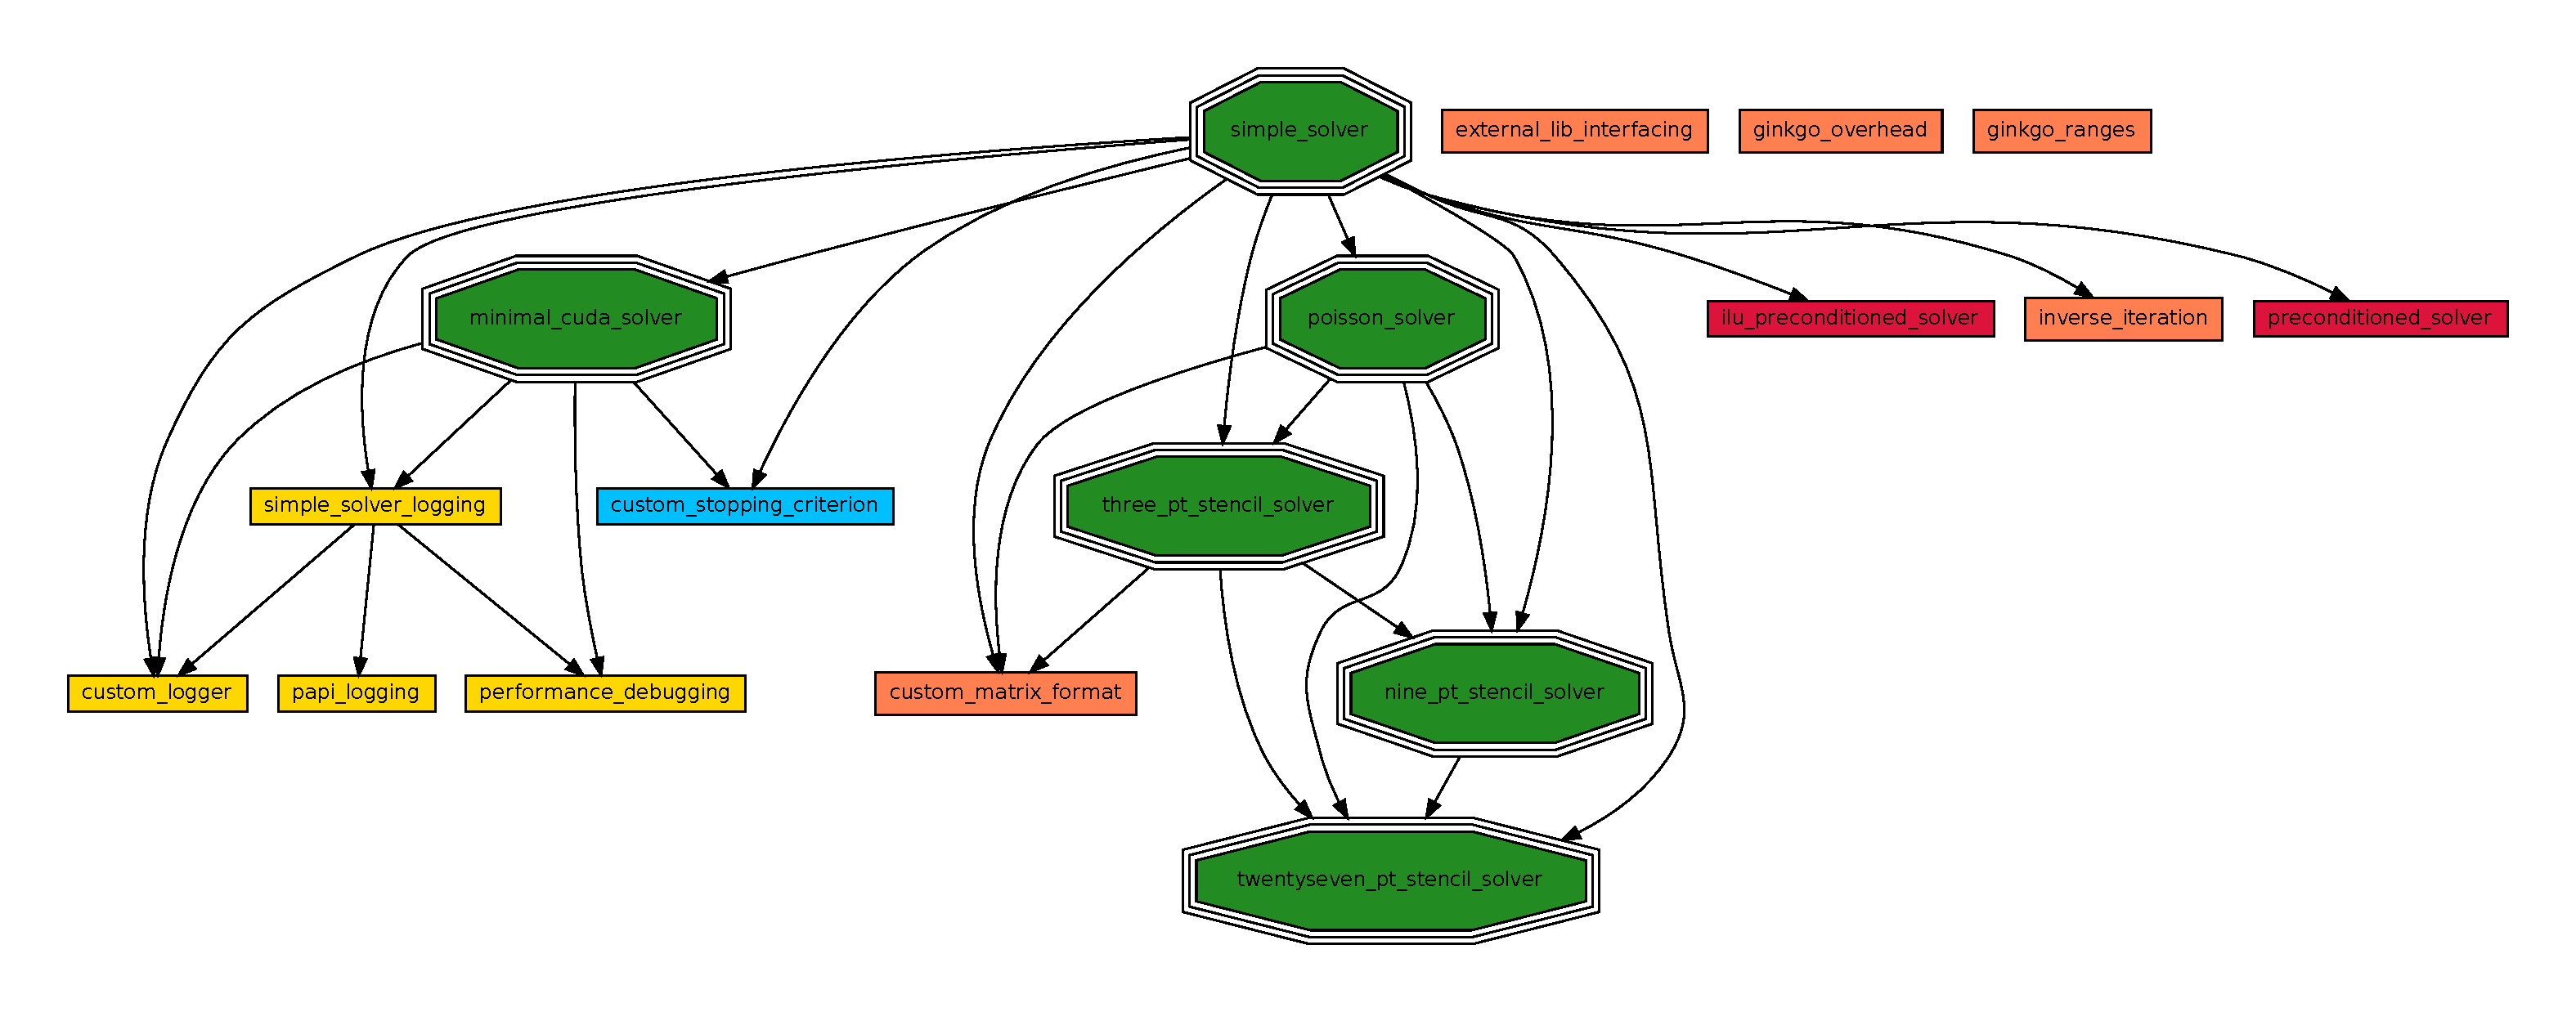
\includegraphics[width=\textwidth,height=\textheight/2,keepaspectratio=true]{dot_inline_dotgraph_1}}
\end{DoxyImageNoCaption}


{\bfseries Legend\+:}~\newline
 
\begin{DoxyImageNoCaption}
  \mbox{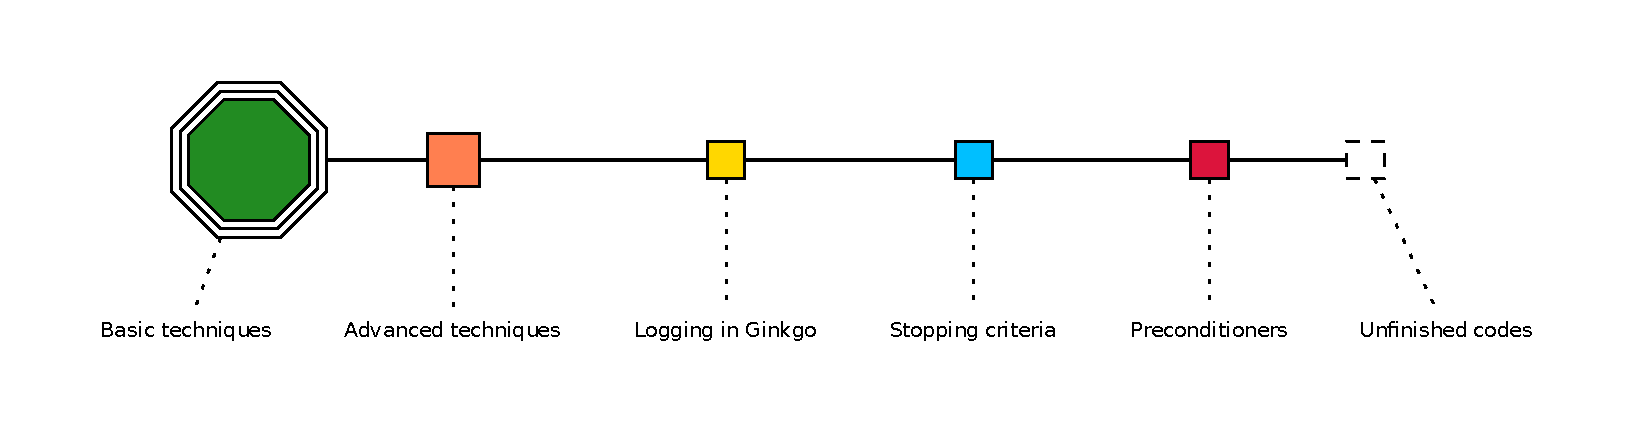
\includegraphics[width=\textwidth,height=\textheight/2,keepaspectratio=true]{dot_inline_dotgraph_2}}
\end{DoxyImageNoCaption}


\label{_list}%
 \subsubsection*{Example programs }

\tabulinesep=1mm
\begin{longtabu} spread 0pt [c]{*{2}{|X[-1]}|}
\hline
\hyperlink{simple_solver}{The simple-\/solver program} &A minimal CG solver in Ginkgo, which reads a matrix from a file. 

\\\cline{1-2}
\hyperlink{minimal_cuda_solver}{The minimal-\/cuda-\/solver program} &A minimal solver on the C\+U\+DA executor than can be run on N\+V\+I\+D\+IA G\+PU\textquotesingle{}s. 

\\\cline{1-2}
\hyperlink{poisson_solver}{The poisson-\/solver program} &Solve an actual physically relevant problem, the poisson problem. The matrix is generated within Ginkgo. 

\\\cline{1-2}
\hyperlink{preconditioned_solver}{The preconditioned-\/solver program} &Using a Jacobi preconditioner to solve a linear system. 

\\\cline{1-2}
\hyperlink{three_pt_stencil_solver}{The three-\/pt-\/stencil-\/solver program} &Using a three point stencil to solve the poisson equation with array views. 

\\\cline{1-2}
\hyperlink{nine_pt_stencil_solver}{The nine-\/pt-\/stencil-\/solver program} &Using a nine point 2D stencil to solve the poisson equation with array views. 

\\\cline{1-2}
\hyperlink{twentyseven_pt_stencil_solver}{The twentyseven-\/pt-\/stencil-\/solver program} &Using a twentyseven point 3D stencil to solve the poisson equation with array views. 

\\\cline{1-2}
\hyperlink{external_lib_interfacing}{The external-\/lib-\/interfacing program} &Using Ginkgo\textquotesingle{}s solver with the external library deal.\+II. 

\\\cline{1-2}
\hyperlink{custom_logger}{The custom-\/logger program} &Creating a custom logger specifically for comparing the recurrent and the real residual norms. 

\\\cline{1-2}
\hyperlink{custom_matrix_format}{The custom-\/matrix-\/format program} &Creating a matrix-\/free stencil solver by using Ginkgo\textquotesingle{}s advanced methods to build your own custom matrix format. 

\\\cline{1-2}
\hyperlink{inverse_iteration}{The inverse-\/iteration program} &Using Ginkgo to compute eigenvalues of a matrix with the inverse iteration method. 

\\\cline{1-2}
\hyperlink{simple_solver_logging}{The simple-\/solver-\/logging program} &Using the logging functionality in Ginkgo to get solver and other information to diagnose and debug your code. 

\\\cline{1-2}
\hyperlink{papi_logging}{The papi-\/logging program} &Using the P\+A\+PI logging library in Ginkgo to get advanced information about your code and its behaviour. 

\\\cline{1-2}
\hyperlink{ginkgo_overhead}{The ginkgo-\/overhead program} &Measuring the overhead of the Ginkgo library. 

\\\cline{1-2}
\hyperlink{custom_stopping_criterion}{The custom-\/stopping-\/criterion program} &Creating a custom stopping criterion for the iterative solution process. 

\\\cline{1-2}
\hyperlink{ginkgo_ranges}{The ginkgo-\/ranges program} &Using the ranges concept to factorize a matrix with the LU factorization. 

\\\cline{1-2}
\end{longtabu}


\label{_topic}%
 \subsubsection*{Example programs grouped by topics}

\paragraph*{{\bfseries Basic techniques}}

\tabulinesep=1mm
\begin{longtabu} spread 0pt [c]{*{2}{|X[-1]}|}
\hline
Solving a simple linear system with choice of executors.  &\hyperlink{simple_solver}{The simple-\/solver program}  

\\\cline{1-2}
Using the C\+U\+DA executor  &\hyperlink{minimal_cuda_solver}{The minimal-\/cuda-\/solver program}  

\\\cline{1-2}
Using preconditioners  &\hyperlink{preconditioned_solver}{The preconditioned-\/solver program}  

\\\cline{1-2}
Solving a physically relevant problem  &\hyperlink{poisson_solver}{The poisson-\/solver program}, \hyperlink{three_pt_stencil_solver}{The three-\/pt-\/stencil-\/solver program}, \hyperlink{nine_pt_stencil_solver}{The nine-\/pt-\/stencil-\/solver program}, \hyperlink{twentyseven_pt_stencil_solver}{The twentyseven-\/pt-\/stencil-\/solver program}, \hyperlink{custom_matrix_format}{The custom-\/matrix-\/format program}  

\\\cline{1-2}
Reading in a matrix and right hand side from a file.  &\hyperlink{simple_solver}{The simple-\/solver program}, \hyperlink{minimal_cuda_solver}{The minimal-\/cuda-\/solver program}, \hyperlink{preconditioned_solver}{The preconditioned-\/solver program}, \hyperlink{inverse_iteration}{The inverse-\/iteration program}, \hyperlink{simple_solver_logging}{The simple-\/solver-\/logging program}, \hyperlink{papi_logging}{The papi-\/logging program}, \hyperlink{custom_stopping_criterion}{The custom-\/stopping-\/criterion program}, \hyperlink{custom_logger}{The custom-\/logger program}  

\\\cline{1-2}
\end{longtabu}


\paragraph*{{\bfseries Advanced techniques}}

\tabulinesep=1mm
\begin{longtabu} spread 0pt [c]{*{2}{|X[-1]}|}
\hline
Using Ginkgo with external libraries.  &\hyperlink{external_lib_interfacing}{The external-\/lib-\/interfacing program}  

\\\cline{1-2}
Customizing Ginkgo  &\hyperlink{custom_logger}{The custom-\/logger program}, \hyperlink{custom_stopping_criterion}{The custom-\/stopping-\/criterion program}, \hyperlink{custom_matrix_format}{The custom-\/matrix-\/format program}  

\\\cline{1-2}
Writing your own matrix format  &\hyperlink{custom_matrix_format}{The custom-\/matrix-\/format program}  

\\\cline{1-2}
Using Ginkgo to construct more complex linear algebra routines.  &\hyperlink{inverse_iteration}{The inverse-\/iteration program}  

\\\cline{1-2}
Logging within Ginkgo.  &\hyperlink{simple_solver_logging}{The simple-\/solver-\/logging program}, \hyperlink{papi_logging}{The papi-\/logging program}, \hyperlink{custom_logger}{The custom-\/logger program}  

\\\cline{1-2}
Constructing your own stopping criterion.  &\hyperlink{custom_stopping_criterion}{The custom-\/stopping-\/criterion program}  

\\\cline{1-2}
Using ranges in Ginkgo.  &\hyperlink{ginkgo_ranges}{The ginkgo-\/ranges program}   \\\cline{1-2}
\end{longtabu}
